% ############### 2.4) RUNTIME VIEW ####################

For letting diagram simpler, we supposed that all the example below are operations of success version (without considering any exceptions, every actor inserts the data correctly and satisfies their authorization requirements).
\newline
Additionally we also note that API gateway does a communication with authorization server to generate a token to let users execute only the ones they have permission to do. 


\begin{figure}[H]
	\centering
    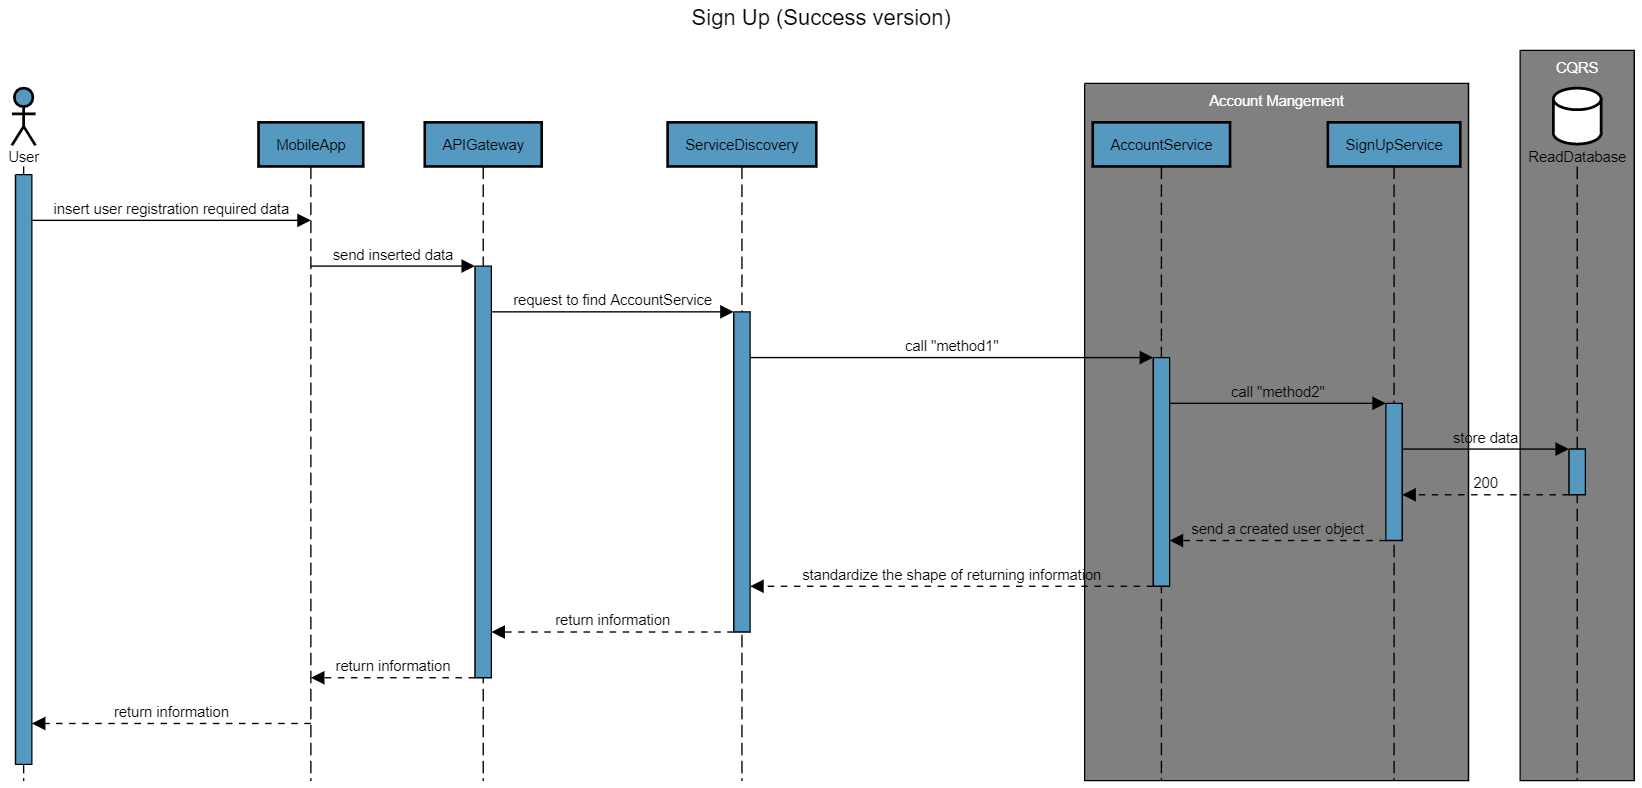
\includegraphics[width=\textwidth]{Images/sequence-diagram/sign-up.png}
	\caption{\label{fig:se_sign_up}Sign Up}
\end{figure}
Actor: All type of user
\newline
UI flow: {\ref{sec:user_mobile_interface} Sign Up, Login}

Firstly this diagram explains the flow of sign up for all type of user. 
Due to CQRS pattern, there are two different database according to their purpose (\ref{sec:component_view}). 
\newline
\textsc{\textcolor{blue}{flow overview}}

Mobile App sends a method ”postUser()” to Mobile Api Gateway, then service discovery does a job to find a routing path by URL of REST api.
Then SignUpService receives post request, after that for updating the database, since it is write operation, it sends command to Command handler to insert the data into Command DB. 

\newpage
\begin{figure}[H]
	\centering
    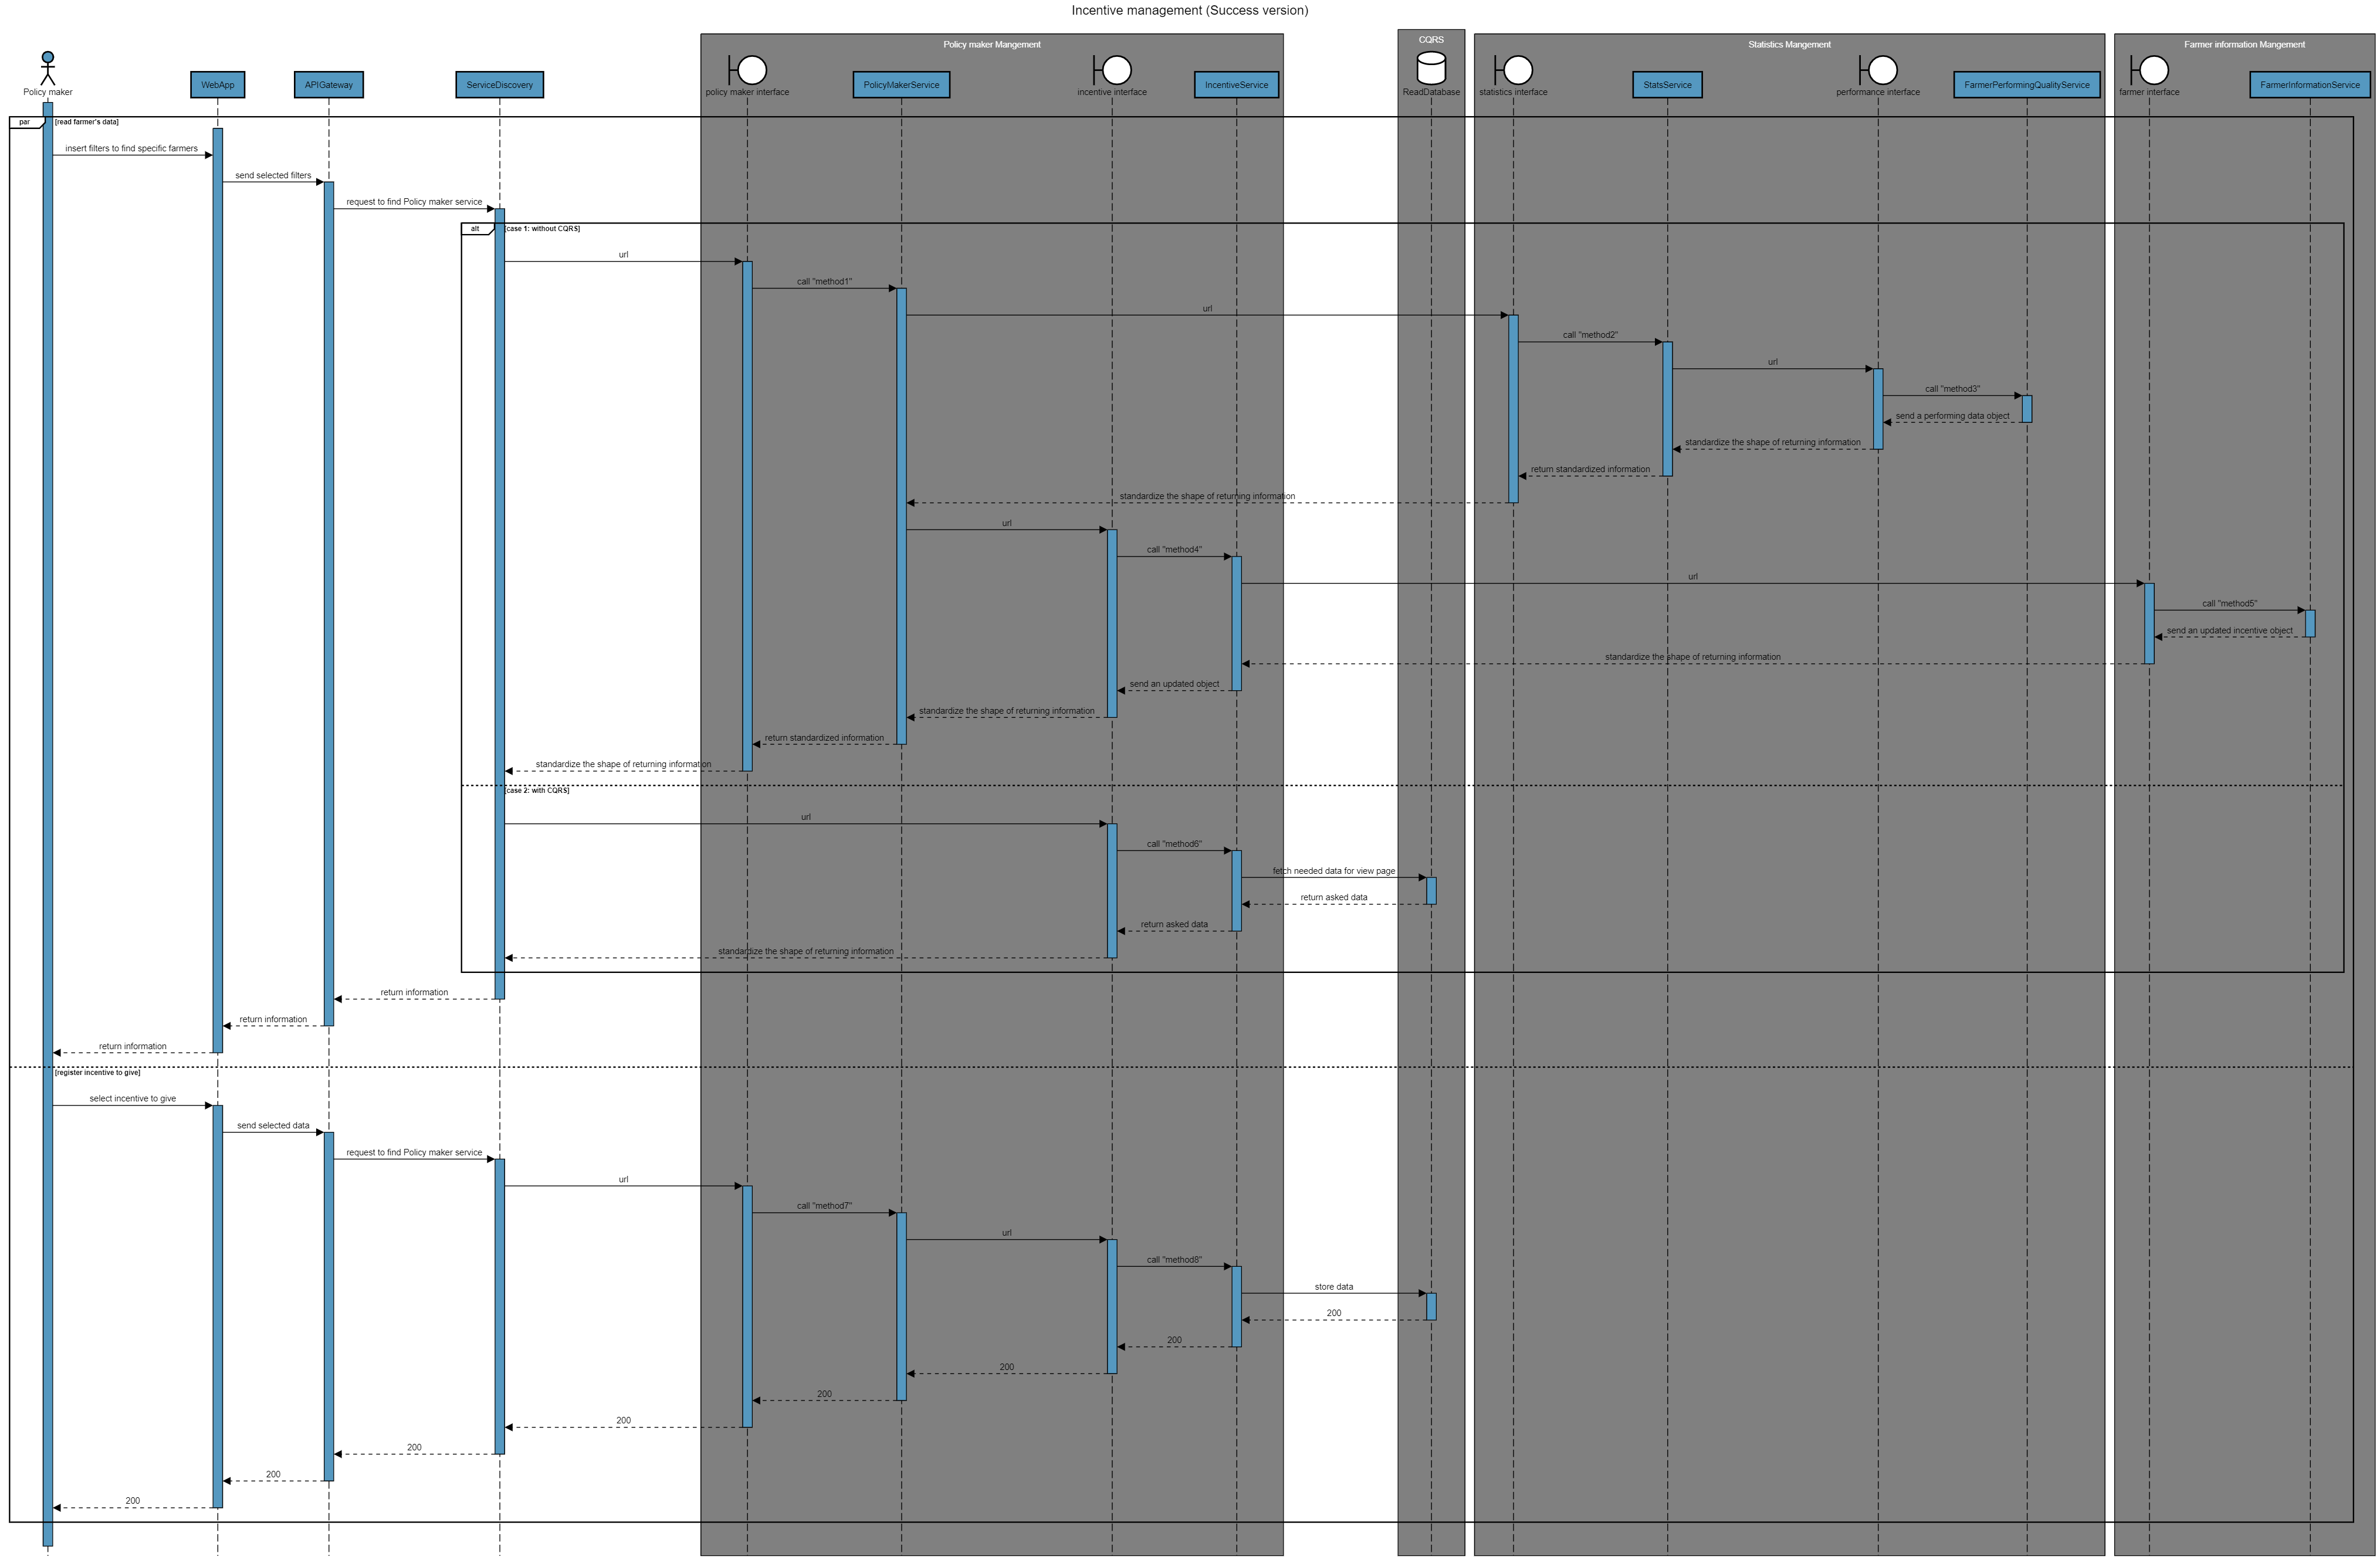
\includegraphics[width=\textwidth]{Images/sequence-diagram/incentive-management.png}
	\caption{\label{fig:se_incentive}Incentive management}
\end{figure}
Actor: Policy maker
\newline
UI flow: {\ref{sec:pm_web_interface} Farmer's performance data}

Secondly on this diagram, we would like to highlight about the reasoning of our design decision. We utilized CQRS pattern though, here it shows a comparison of each flow, one with CQRS pattern architecture, another without it.
By the fact we consider the analysis part taken cared by 3rd party systems, it also suits to have replica of database to fetch aggregated data when it is needed regardless of condition of their system.
\newline
\textsc{\textcolor{blue}{flow overview}}
\newline
Above part describes the flow of read operation. Search and show the data from database, it is required to access Query DB.
Then the below part explains the flow of write operation.
Incentive service needs to call Notification service to let the farmer who is selected to receive it.

\newpage
\begin{figure}[H]
	\centering
    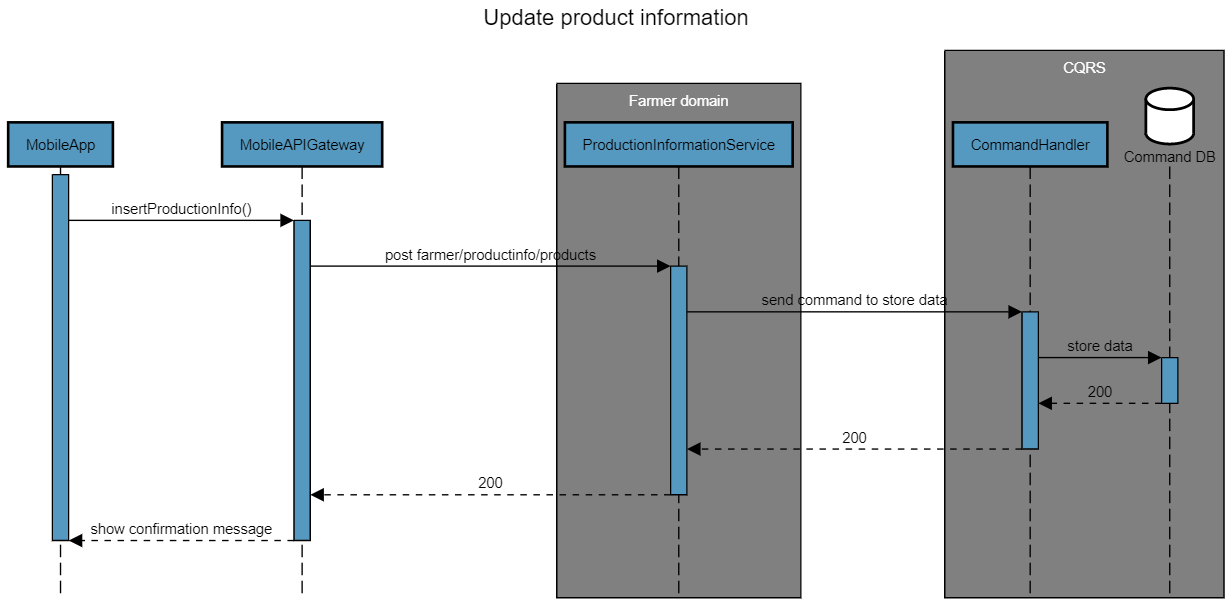
\includegraphics[width=\textwidth]{Images/sequence-diagram/product-info.png}
	\caption{\label{fig:se_product}Product information registration}
\end{figure}
Actor: Farmer
\newline
UI flow: {\ref{sec:farmer_mob_interface} Production data registration, Help/Suggestion request}

From this diagram, we consider API gateway component contains the operation to communicate with discovery service to find the suitable service location, besides that we also expect that each service has interfaces right before receiving a request as they are shown in two examples above (sign up, incentive management).
\newline
\textsc{\textcolor{blue}{flow overview}}
\newline
Farmer inserts needed information and send the production data to register it. API gateway contacts to authorization server to assure the permission, if it is verified, then discovery service finds ProductInformationService and execute the method. Since it is write operation, it sends data to Command handler to insert into Command DB.  

\newpage
\begin{figure}[H]
	\centering
    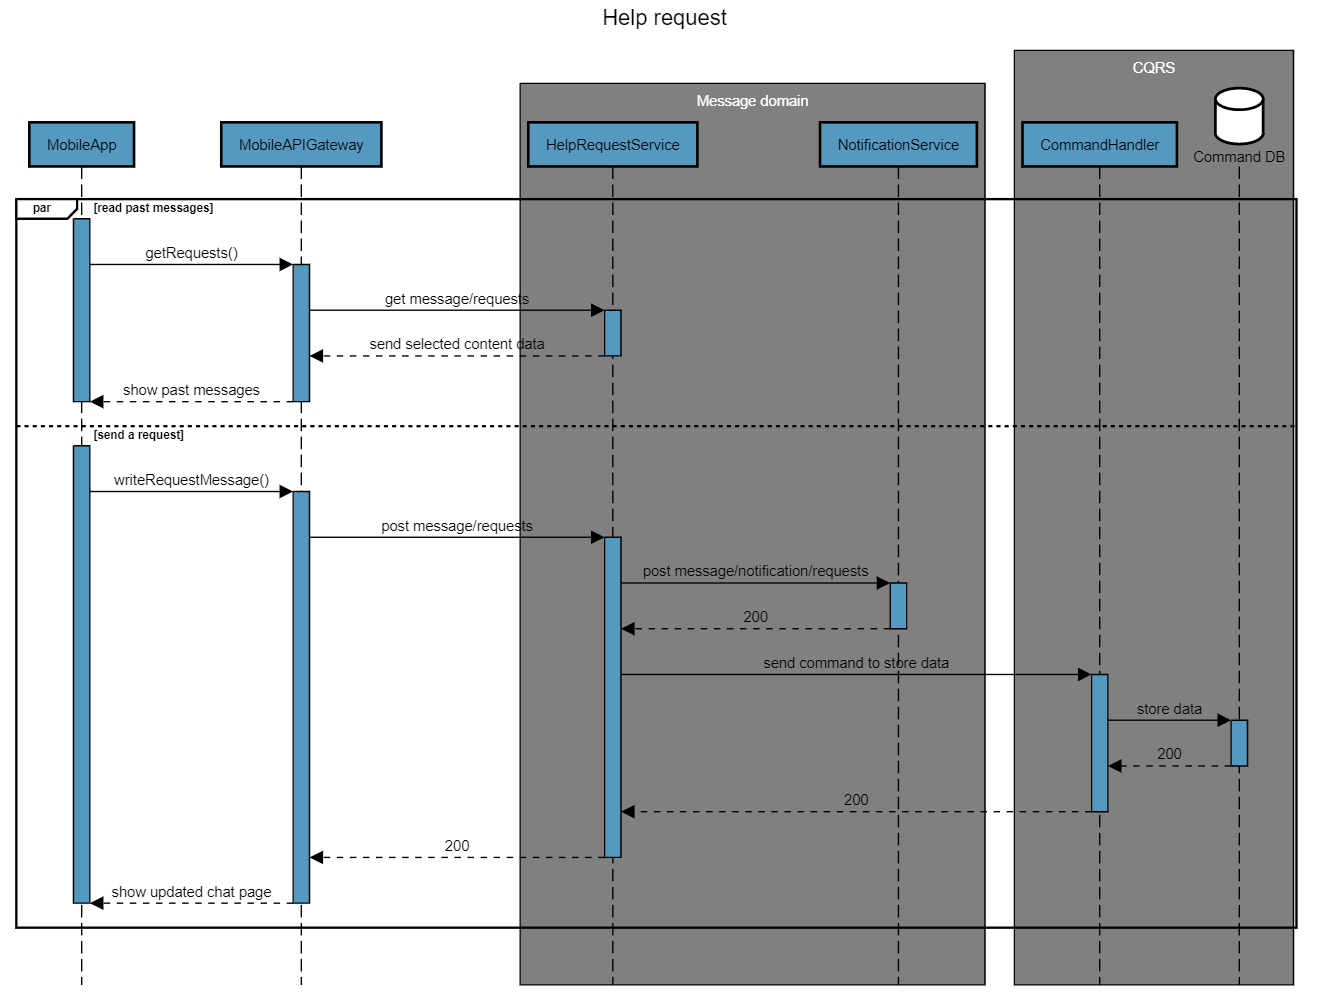
\includegraphics[width=\textwidth]{Images/sequence-diagram/help-request.png}
	\caption{\label{fig:se_help}Help request registration}
\end{figure}
Actor: Farmer
\newline
UI flow: {\ref{sec:farmer_mob_interface} Production data registration, Help/Suggestion request}

This diagram explains the flow of asking help request.
As a previous step, it requires farmer to select whom they would like to ask though, we assumed this operation has been done in advance and the diagram above describes the phase afterwards.
\newline
\textsc{\textcolor{blue}{flow overview}}
\newline
First half shows the flow of read operation to visualise the past messages, on the other hand the below part represents the write operation to send the message. 
For read operation it does not access to Query DB since the data is not aggregated data, it simply access the database inside of own service.

\newpage
\begin{figure}[H]
	\centering
    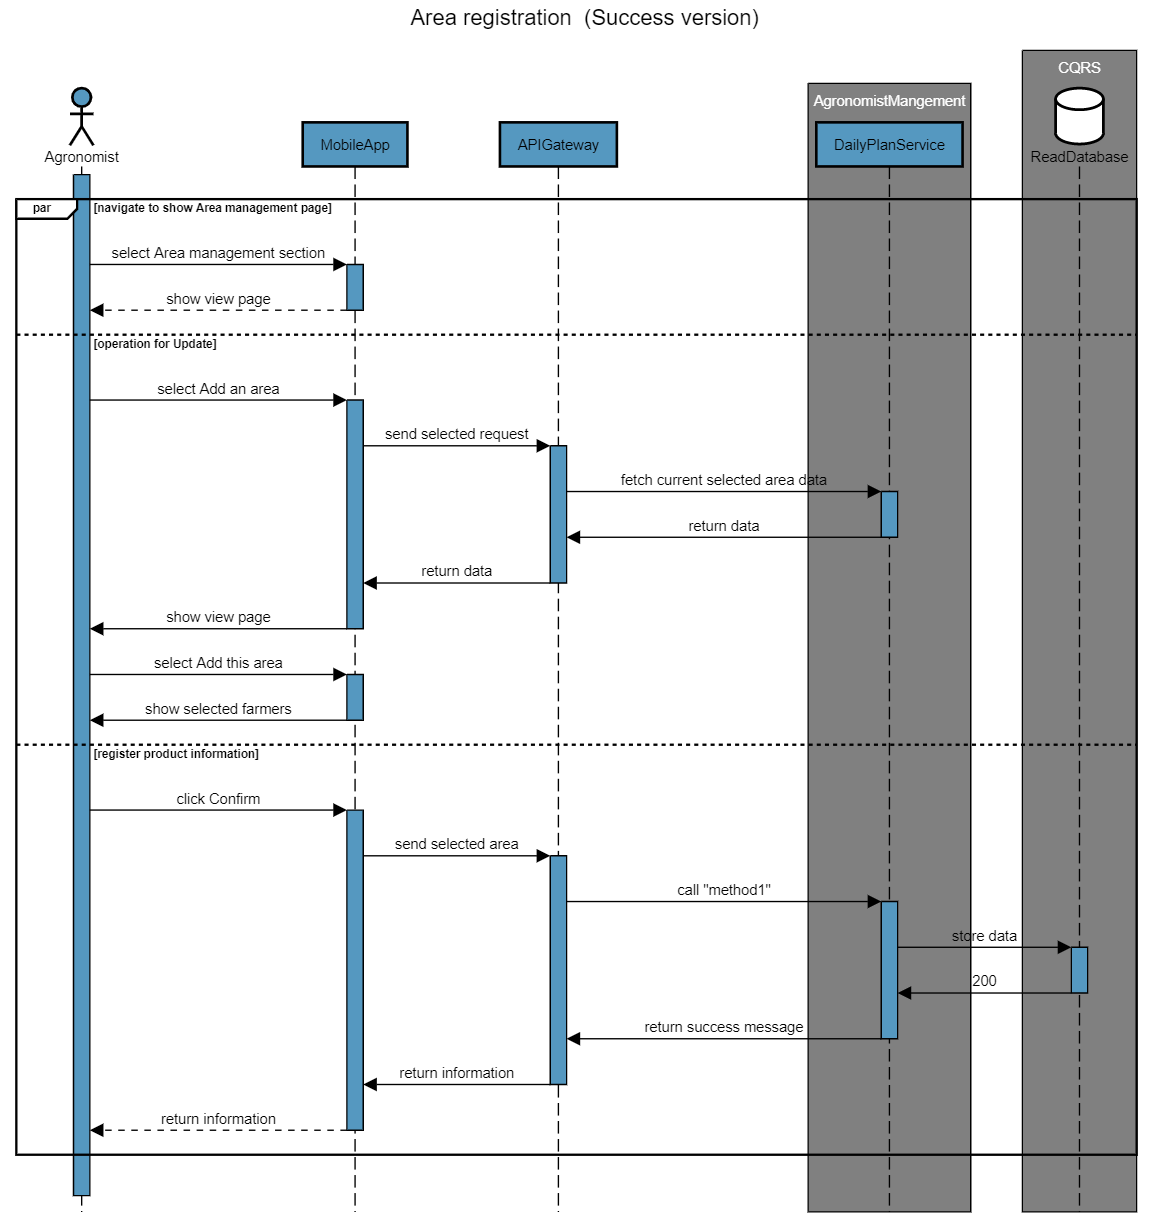
\includegraphics[width=\textwidth]{Images/sequence-diagram/area-registration.png}
	\caption{\label{fig:se_area}Area registration}
\end{figure}
Actor: Agronomist
\newline
UI flow: {\ref{sec:agronomist_mob_interface} Area management}

This diagram shows the flow of registering new area to supervise. As like other examples, this diagram contains read and write operation individually.

\textsc{\textcolor{blue}{flow overview}}
\newline
Firstly by calling getAreas(), it will fetch current area information about the place(name of farmers, agronomist). After agronomist observe area information and if they are interested in they could register a new area to supervise it. Write operation require to update Command DB to let new registered data be reachable by other services.

\newpage
\begin{figure}[H]
	\centering
    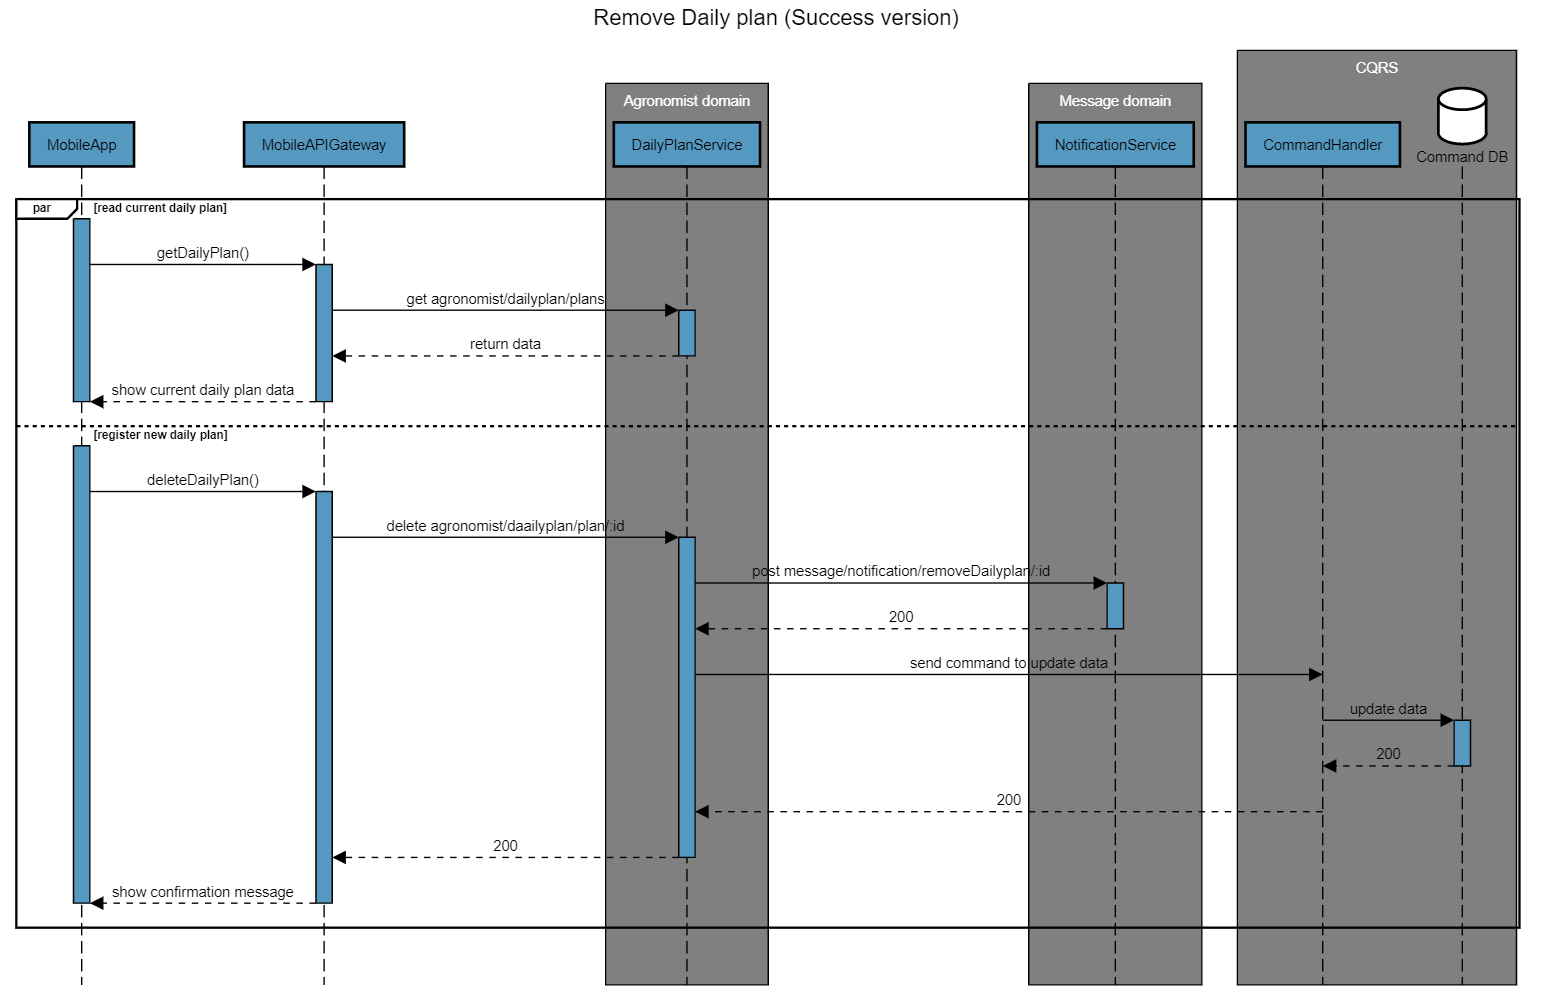
\includegraphics[width=\textwidth]{Images/sequence-diagram/daily-plan.png}
	\caption{\label{fig:se_daily}Remove Daily plan}
\end{figure}
Actor: Agronomist
\newline
UI flow: {\ref{sec:agronomist_mob_interface} Daily plan management}

As a last example, this diagram shows the flow of updating daily plan of agronomist.
Unlike other insertion examples, here it deletes the record from database, so it requires DELETE method.
\newline
\textsc{\textcolor{blue}{flow overview}}
\newline
On the upper part it let agronomist know the daily plan they have. Instead, the bottom explains the flow of deletion operation. Specifying id in url, Command Handler searches the record owns that id and it deletes the one matches. 